%==============================================================================
% Chapitre 24 - Géométrie des projectiles
%==============================================================================

\section{Introduction}

La géométrie d'un projectile influence directement son comportement
aérodynamique.

Sa forme détermine notamment :

\begin{itemize}
    \item la traînée ;
    \item la stabilité ;
    \item la conservation de vitesse ;
    \item la portée ;
    \item la sensibilité au vent.
\end{itemize}

Les projectiles modernes résultent de plusieurs siècles d'évolution visant à
optimiser ces caractéristiques.

\begin{aretenir}

La géométrie constitue l'un des principaux facteurs influençant les
performances balistiques d'un projectile.

\end{aretenir}

\section{Description générale}

Un projectile moderne peut être décomposé en plusieurs zones principales :

\begin{itemize}
    \item la pointe ;
    \item l'ogive ;
    \item le corps cylindrique ;
    \item le culot.
\end{itemize}

Chaque zone possède une fonction aérodynamique particulière.

\begin{figure}[htbp]
\centering
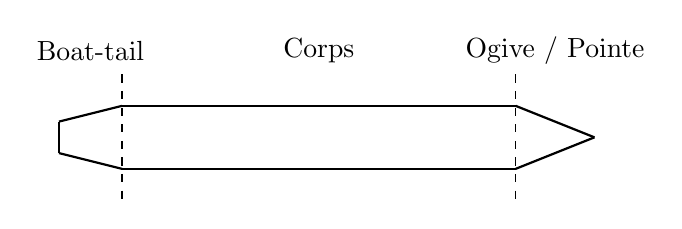
\begin{tikzpicture}[scale=1]

% Corps
\draw[thick] (0,0.4) -- (5,0.4);
\draw[thick] (0,-0.4) -- (5,-0.4);

% Pointe
\draw[thick] (5,0.4) -- (6,0);
\draw[thick] (5,-0.4) -- (6,0);

% Boat-tail
\draw[thick] (-0.8,0.2) -- (0,0.4);
\draw[thick] (-0.8,-0.2) -- (0,-0.4);
\draw[thick] (-0.8,0.2) -- (-0.8,-0.2);

% Labels
\draw[dashed] (0,0.8) -- (0,-0.8);
\draw[dashed] (5,0.8) -- (5,-0.8);

\node at (-0.4,1.1) {Boat-tail};
\node at (2.5,1.1) {Corps};
\node at (5.5,1.1) {Ogive / Pointe};

\end{tikzpicture}
\caption{Géométrie simplifiée d'un projectile moderne.}
\label{fig:geometrie_projectile}
\end{figure}

\section{La pointe}

La pointe constitue l'extrémité avant du projectile.

Sa géométrie influence fortement :

\begin{itemize}
    \item la pénétration dans l'air ;
    \item la génération d'ondes de choc ;
    \item la traînée.
\end{itemize}

On distingue notamment :

\begin{itemize}
    \item les pointes arrondies ;
    \item les pointes ogivales ;
    \item les pointes très effilées ;
    \item les pointes tronquées.
\end{itemize}

\section{L'ogive}

L'ogive est la partie profilée reliant la pointe au corps cylindrique.

Elle joue un rôle majeur dans la réduction de la traînée.

Les formes les plus courantes sont :

\begin{itemize}
    \item tangentielle ;
    \item sécante ;
    \item hybride.
\end{itemize}

Ces profils seront réétudiés lors des chapitres consacrés à l'aérodynamique.

\section{Le corps cylindrique}

Le corps cylindrique constitue la partie centrale du projectile.

Son diamètre correspond généralement au calibre nominal.

Cette zone assure notamment :

\begin{itemize}
    \item le guidage dans le canon ;
    \item la prise de rayures ;
    \item une partie de la stabilité aérodynamique.
\end{itemize}

\section{Le culot}

Le culot constitue la partie arrière du projectile.

Cette zone influence fortement la traînée de culot.

Pendant longtemps, les projectiles possédaient un culot plat.

Les conceptions modernes utilisent souvent des formes optimisées.

\section{Boat-tail}

Un projectile à culot rétreint est souvent désigné par le terme anglais
\emph{boat-tail}.

Sa partie arrière présente une réduction progressive du diamètre.

Cette géométrie permet généralement :

\begin{itemize}
    \item une diminution de la traînée ;
    \item une meilleure conservation de vitesse ;
    \item une portée accrue.
\end{itemize}

\begin{aretenir}

Le boat-tail est l'une des améliorations aérodynamiques les plus importantes
des projectiles modernes.

\end{aretenir}

\section{Méplat}

Le méplat correspond à la surface située à l'extrémité avant du projectile.

Selon les conceptions, il peut être :

\begin{itemize}
    \item quasi inexistant ;
    \item volontairement important ;
    \item modifié pour répondre à un besoin spécifique.
\end{itemize}

Le méplat influence les performances aérodynamiques.

\section{Longueur}

La longueur constitue une caractéristique essentielle.

Deux projectiles de même calibre peuvent présenter des longueurs très
différentes.

Cette dimension influence notamment :

\begin{itemize}
    \item la stabilité ;
    \item la masse ;
    \item le centre de gravité ;
    \item le choix du pas de rayure.
\end{itemize}

\section{Diamètre}

Le diamètre du projectile est généralement associé au calibre.

Il influence :

\begin{itemize}
    \item la surface frontale ;
    \item la traînée ;
    \item la masse potentielle ;
    \item les performances terminales.
\end{itemize}

\section{Allongement}

L'allongement correspond au rapport entre :

\begin{equation}
\lambda=\frac{L}{D}
\end{equation}

où :

\begin{itemize}
    \item $L$ représente la longueur ;
    \item $D$ représente le diamètre.
\end{itemize}

Cette grandeur est largement utilisée en aérodynamique.

\begin{aretenir}

À calibre identique, un projectile plus long possède généralement un
allongement plus élevé.

\end{aretenir}

\section{Surface frontale}

La surface frontale correspond à la section maximale du projectile.

Pour un projectile cylindrique :



Cette surface intervient directement dans les équations de traînée.

\section{Influence de la forme sur la traînée}

Deux projectiles de même masse peuvent présenter des comportements très
différents selon leur géométrie.

Une forme mieux profilée permet généralement :

\begin{itemize}
    \item une réduction de la traînée ;
    \item un temps de vol plus faible ;
    \item une meilleure conservation d'énergie.
\end{itemize}

\section{Influence de la forme sur la stabilité}

La géométrie influence également :

\begin{itemize}
    \item le centre de gravité ;
    \item le centre de pression ;
    \item les moments aérodynamiques.
\end{itemize}

Ces notions seront étudiées dans les prochains chapitres.

\section{Familles de formes}

Les géométries les plus courantes sont :

\begin{itemize}
    \item sphérique ;
    \item cylindro-ogivale ;
    \item boat-tail ;
    \item empennée ;
    \item flèche.
\end{itemize}

Chaque famille répond à des contraintes particulières.

\section{Géométrie et simulation}

Dans les modèles balistiques simples, la géométrie est souvent représentée
par quelques paramètres seulement.

Les modèles avancés utilisent :

\begin{itemize}
    \item le profil complet ;
    \item les centres caractéristiques ;
    \item les coefficients aérodynamiques.
\end{itemize}

La fidélité de la simulation dépend fortement de la qualité de cette
description géométrique.

\begin{simulation}

Les modèles de type 6DOF utilisent souvent des données géométriques très
détaillées du projectile.

\end{simulation}

\section{Vers les chapitres suivants}

Après avoir étudié la forme extérieure du projectile, nous nous
intéresserons à sa constitution interne :

\begin{itemize}
    \item masse ;
    \item matériaux ;
    \item répartition des masses ;
    \item centres caractéristiques.
\end{itemize}

Ces éléments permettront ensuite de comprendre les phénomènes de stabilité.

\section{À retenir}

\begin{aretenir}

\begin{itemize}
    \item La géométrie influence directement les performances balistiques.
    \item L'ogive et le culot jouent un rôle majeur dans la traînée.
    \item Le boat-tail améliore généralement les performances aérodynamiques.
    \item L'allongement est une caractéristique importante des projectiles.
    \item La forme influence la stabilité future du projectile.
\end{itemize}

\end{aretenir}
